Реализация модели вычислений с помощью понятия машины Тьюринга.

При построении математической модели алгоритма Пост и 
Тьюринг исходили из того, что все действия, которые может 
производить любой алгоритм, можно разложить на некоторые 
канонические элементарные шаги, выполняемые подходяще 
устроенными вычислительными машинами. 

Такие машины схематически определяются следующим образом.

\subsection*{Схематическое описание работы машины Тьюринга}
\begin{figure}[H]
    \centering
    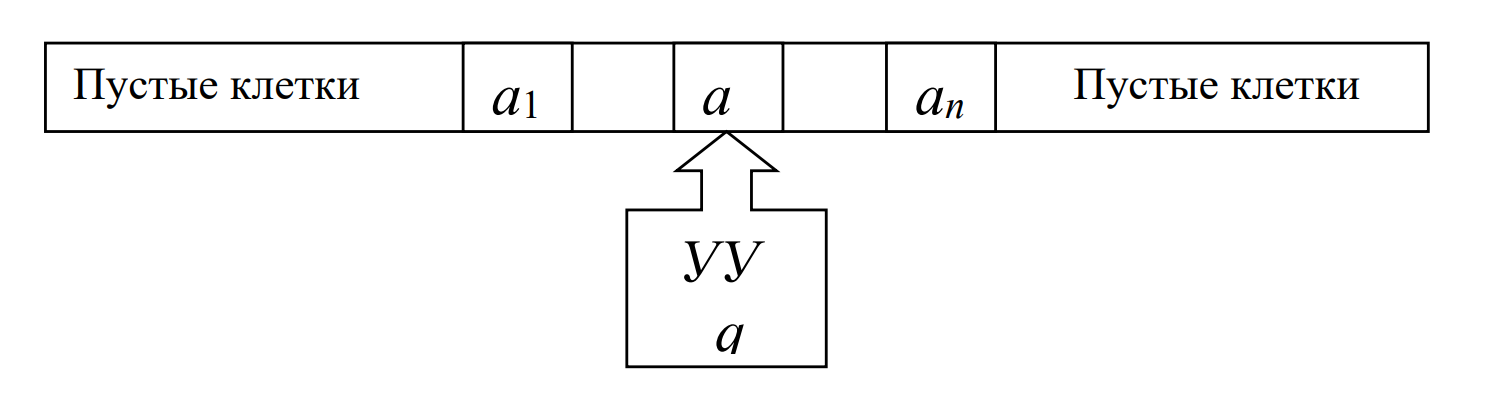
\includegraphics[height = 3cm]{images/machine.png}
\end{figure}

\begin{enumerate}
    \item Символы внешнего алфавита $\Sigma=\{0,1,\ldots\}$ записываются в ячейки конечной ленты, которая называется \textit{внешней памятью машины}, при необходимости в ячейки записывается символ *, который называется \textit{пустым}
    \item Символы внутреннего алфавита $Q = \{q_S,q_F,\ldots\}$ обозначают состояния \textit{управляющего устройства машины (УУ)} с \textit{просматривающей головкой}, которая может перемещаться вдоль ленты и в каждый момент времени $t$ просматривать одну ячейку
    \item \textit{Программа машины}
    $$\Pi = \{T()\}$$
\end{enumerate}